\documentclass[12pt,mathserif,professionalfont]{beamer}

\mode<presentation>{%
    \usetheme[alternativetitlepage=bild]{Rub}
    \titlegraphic{data/flickr/img-bg.jpg}
    \sponsorlogo[height=15mm]{img-gdata.pdf}

    \setbeamercovered{transparent}
}
\usepackage{pgfpages}
\setbeameroption{show notes on second screen}

\usepackage[utf8]{inputenc}
\usepackage[T1]{fontenc}

\usepackage{rubfonts2009}
\usepackage[scaled=.90]{helvet}
\usepackage{courier}
\usepackage{eulervm}
%\usefonttheme[onlymath]{serif}

\usepackage{abbrv}
\usepackage{delimiters}

\usepackage[english]{babel}
\usepackage{csquotes}

\usepackage{amsmath}
\usepackage{mathtools}

\usepackage{etoolbox,siunitx}
\sisetup{binary-units}

\usepackage{booktabs}

\usepackage{tikz}
\usepackage{tikzsymbols}
\usetikzlibrary{calc}
\usetikzlibrary{positioning}
\usetikzlibrary{decorations.pathreplacing, overlay-beamer-styles}

\tikzset{%
    invisible/.style={opacity=0},
    visible on/.style={alt={#1{}{invisible}}},
    alt/.code args={<#1>#2#3}{%
        \alt<#1>{\pgfkeysalso{#2}}{\pgfkeysalso{#3}} % \pgfkeysalso doesn't change the path
    },
}

\tikzset{%
    marked/.style={%
        fill=blue,
    },
    marked on/.style={alt=#1{marked}{}},
}

\usepackage[beamer]{hf-tikz}
\usepackage{multirow}

\usepackage{media9}

\setbeamertemplate{bibliography item}[text]
\usepackage[%
    backend=biber,
    bibencoding=ascii,
    style=alphabetic,
    sortcites,
    maxbibnames=10,
    maxcitenames=2,
    firstinits=true,
]{biblatex}
\DefineBibliographyStrings{english}{%
    andothers = {\etal/}
}
\DeclareFieldFormat{eprint:iacr}{%
\mkbibacro{iacr}\addcolon\space{}
    \href{https://eprint.iacr.org/#1}{\nolinkurl{#1}}
}
\DeclareFieldFormat{eprint:iacrconf}{%
\mkbibacro{iacr}\addcolon\space{}
    \href{https://www.iacr.org/archive/#1}{\nolinkurl{#1}}
}
\renewcommand\bibfont{\scriptsize}
\bibliography{bibliography}

\newcommand{\blfootnote}[1]{%
    \begingroup
        \renewcommand\thefootnote{}\footnote{#1}%
        \addtocounter{footnote}{-1}%
    \endgroup
}

\makeatletter
\def\maxwidth#1{\ifdim\Gin@nat@width>#1 #1\else\Gin@nat@width\fi}
\def\maxheight#1{\ifdim\Gin@nat@height>#1 #1\else\Gin@nat@height\fi}
\makeatother

\title{Attacks on Lattice Crypto}
\subtitle{}
\author[Friedrich~Wiemer]{Friedrich~Wiemer}
\institute{%
    FluxFingers\\[0.5em]
    Workgroup Symmetric Cryptography\\
    Ruhr University Bochum
}

\date{December 7th, 2016}

\AtBeginSection[]

\begin{document}

\begin{frame}
    \titlepage{}
\end{frame}

%\begin{frame}{Outline}
%    \tableofcontents
%\end{frame}

\section{The WSN construction}
\begin{frame}{Block Ciphers}
    \centering
    \begin{tikzpicture}
    \only<1>{%
        \begin{scope}
            \node (title) [xshift=70pt, yshift=95pt] {Encrypt plaintext in blocks $p_i$ of $n$ bits, under a key of $n$ bits:};

            \node (f0) at ($0*(5cm,0)$) [minimum size=4cm,rounded corners=1ex,fill=black!80!white,draw] {{\sc \textcolor{white}{Enc}}};
            \node (m0) [above of=f0, node distance=2.75cm] {$p_0 \in \set{0,1}^n$};
            \node (k0) [left of=f0, node distance=3.5cm] {$k \in \set{0,1}^n$};
            \node (c0) [below of=f0, node distance=2.75cm] {$c_0 \in \set{0,1}^n$};
            \draw[-latex, thick] (m0) -- (f0);
            \draw[-latex, thick] (k0) -- (f0);
            \draw[-latex, thick] (f0) -- (c0);

            \node (f1) at ($1*(5cm,0)$) [minimum size=4cm,rounded corners=1ex,fill=black!80!white,draw] {{\sc \textcolor{white}{Enc}}};
            \node (m1) [above of=f1, node distance=2.75cm] {$p_1 \in \set{0,1}^n$};
            \node (k1) [right of=f1, node distance=3.5cm] {$k \in \set{0,1}^n$};
            \node (c1) [below of=f1, node distance=2.75cm] {$c_1 \in \set{0,1}^n$};
            \draw[-latex, thick] (m1) -- (f1);
            \draw[-latex, thick] (k1) -- (f1);
            \draw[-latex, thick] (f1) -- (c1);
        \end{scope}
    }
    \visible<1->{%
    \note{%
    \begin{itemize}
        \item<1-> Block ciphers encrypt \emph{blocks} of $n$-bit inputs under an $n$-bit master key
        \item<1-> As a basic cryptographic primitive, we need special modes of operations, if the data to be encrypted is not of exactly $n$-bit length.
        \item<1-> This we do not consider here, instead we want to look at how to build this black box.
    \end{itemize}
    }
    }
    \only<2>{%
        \begin{scope}[opacity=0.2]
            \node (title) [xshift=70pt, yshift=95pt] {Encrypt plaintext in blocks $p_i$ of $n$ bits, under a key of $n$ bits:};

            \node (f0) at ($0*(5cm,0)$) [minimum size=4cm,rounded corners=1ex,fill=black!80!white,draw] {{\sc \textcolor{white}{Enc}}};
            \node (m0) [above of=f0, node distance=2.75cm] {$p_0 \in \set{0,1}^n$};
            \node (k0) [left of=f0, node distance=3.5cm] {$k \in \set{0,1}^n$};
            \node (c0) [below of=f0, node distance=2.75cm] {$c_0 \in \set{0,1}^n$};
            \draw[-latex, thick] (m0) -- (f0);
            \draw[-latex, thick] (k0) -- (f0);
            \draw[-latex, thick] (f0) -- (c0);

            \node (f1) at ($1*(5cm,0)$) [minimum size=4cm,rounded corners=1ex,fill=black!80!white,draw] {{\sc \textcolor{white}{Enc}}};
            \node (m1) [above of=f1, node distance=2.75cm] {$p_1 \in \set{0,1}^n$};
            \node (k1) [right of=f1, node distance=3.5cm] {$k \in \set{0,1}^n$};
            \node (c1) [below of=f1, node distance=2.75cm] {$c_1 \in \set{0,1}^n$};
            \draw[-latex, thick] (m1) -- (f1);
            \draw[-latex, thick] (k1) -- (f1);
            \draw[-latex, thick] (f1) -- (c1);
        \end{scope}
        \note{%
        \begin{itemize}
            \item Typicall approach is an SPN structure, where key-addition, S-box layer and a linear layer are iterated over several rounds.
            \item Relatively well understood
            \item Good security arguments against known attacks
            \item There are some problems: differentials and linear hull effects
        \end{itemize}
        }
    }
    \visible<2->{%
        \fill [fill=white, opacity=0.8, rounded corners=1ex] (0, 3.8) rectangle (4.5, -3.2);
        \node (xor-in) [right=37.5pt of m0] {};
        \node (diff-char) [below=-35pt of xor-in, xshift=-6pt] {\includegraphics[height=0.8\textheight]{data/spn}};
    }
    \end{tikzpicture}
\end{frame}

\begin{frame}{The WSN construction}
    \centering
    Published by \href{https://doi.org/10.1007/978-3-662-48800-3_18}{Tessaro at AsiaCrypt 2015} [\texttt{\href{https://ia.cr/2015/868}{ia.cr/2015/868}}].
    \begin{minipage}[t][90pt][t]{0.47\textwidth}
        \begin{block}{Overview round, iterated $r$ times\vpPp}
            \centering
            \vfill
            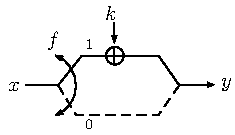
\includegraphics{data/wsn-schematic-1round}
            \vfill
        \end{block}
    \end{minipage}
    \hfill
    \begin{minipage}[t][90pt][t]{0.47\textwidth}
        \begin{block}{Whitened Swap-Or-Not round function}
            \vspace*{-12.5pt}
            \begin{gather*}
                x, k \in \set{0,1}^n \quad\text{and}\quad f_{k} : \set{0,1}^n \to \set{0,1} \\
                y = \begin{cases*}
                    x + k & if $f_{k}(x) = 1$ \\
                    x     & if $f_{k}(x) = 0$
                    \end{cases*}
            \end{gather*}
        \end{block}
    \end{minipage}
    \note{%
    \begin{itemize}
        \item Lets take a look at the WSN construction (simplified).
        \item Again, an iterated round function, where the input is fed into from the left.
        \item Next, a Boolean function decides if either the round key $k$ is xored onto the input, or nothing happens.
        \item The result is the updated state, respective the output of the round.
        \item In other words, $x$, and $k$ are both $n$-bit strings and $f$ is an $n$-bit Boolean function.
        \item The round output $y$ is either $x+k$ if $f_k(x) = 1$ or just $x$ in the other case.
        \item So why is this nice?
    \end{itemize}
    }

    \visible<2->{%
    \begin{minipage}[t][60pt][t]{0.47\textwidth}
        \begin{block}{Properties of $f_{k}$ (needed for decryption)\vpPp}
            \vspace{-5pt}
            \begin{equation*}
                f_k(x) = f_k(x + k)
            \end{equation*}
        \end{block}
    \end{minipage}
    \hfill
    \begin{minipage}[t][60pt][t]{0.47\textwidth}
        \begin{block}{Security Proposition (informal)}
            \centering
            The WSN construction with $r = \mathcal{O}(n)$ rounds is\\
            \emph{Full Domain} secure.
            \vspace{1.5pt}
        \end{block}
    \end{minipage}
    }
    \only<2->{%
    \note{%
    \begin{itemize}
        \item Tessaro was able to show that this construction, when iterated over $\mathcal{O}(n)$ rounds, achieves \emph{Full Domain} security (what ever that means).
        \item One further property of $f$ which we need for decryption is that $x$ and $x+k$ maps to the same output.
    \end{itemize}
    }
}
\end{frame}

\begin{frame}{The WSN construction}{Encryption}
    \centering
    \begin{forest}
        %for tree={grow=east},
        [{\textcolor{green!90!blue}{$x$}},
        name=root,
        for children={visible on=<2->}
            [{$x$},
            for children={visible on=<3->}
                [{$x$},
                for children={visible on=<4->}
                    [{$x$}, name=left node]
                    [{$x + k_2$}]
                ]
                [{$x + k_1$},
                for children={visible on=<4->}
                    [{$x + k_1$}]
                    [{$x + k_1 + k_2$}]
                ]
            ]
            [{\textcolor{green!90!blue}{$x + k_0$}},
            edge={thick, green!90!blue},
            for children={visible on=<3->}
                [{\textcolor{green!90!blue}{$x + k_0$}},
                edge={thick, green!90!blue},
                for children={visible on=<4->}
                    [{$x + k_0$}]
                    [{\textcolor{green!90!blue}{$x + k_0 + k_2$}},
                    edge={thick, green!90!blue}
                    ]
                ]
                [{$x + k_0 + k_1$},
                for children={visible on=<4->}
                    [{$x + k_0 + k_1$}]
                    [{$x + k_0 + k_1 + k_2$}, name=right node]
                ]
            ]
        ]
        \node[above of=root, yshift=-15pt] {Input};
    \end{forest}

    \visible<4->{%
    %\vspace{-15pt}
    \begin{equation*}
        \text{Encryption:}\qquad
        E_{k}(x) \coloneqq x + \sum_{i=1}^{r} \lambda_i k_i = y
    \end{equation*}
    }

    \only<1->{\note{\begin{itemize}
        \item We can observe an interesting first property, when looking at the encryption procedure round by round
        \item Starting with the plaintext $x$\dots
    \end{itemize}}}
    \only<2->{\note{\begin{itemize}
        \item \dots in each round, we either add the round key $k_i$, \dots
    \end{itemize}}}
    \only<3->{\note{\begin{itemize}
        \item \dots or not.
    \end{itemize}}}
    \only<4->{\note{\begin{itemize}
        \item Thus we end up with a binary tree of possible states.
        \item Furthermore, the encryption can also be written as the plaintext plus the sum of some round keys, chosen by the $\lambda_i$'s here.
    \end{itemize}}}

\end{frame}

\begin{frame}{An Implementation}
    \visible<2->{%
    \begin{minipage}{0.40\textwidth}
        \centering
        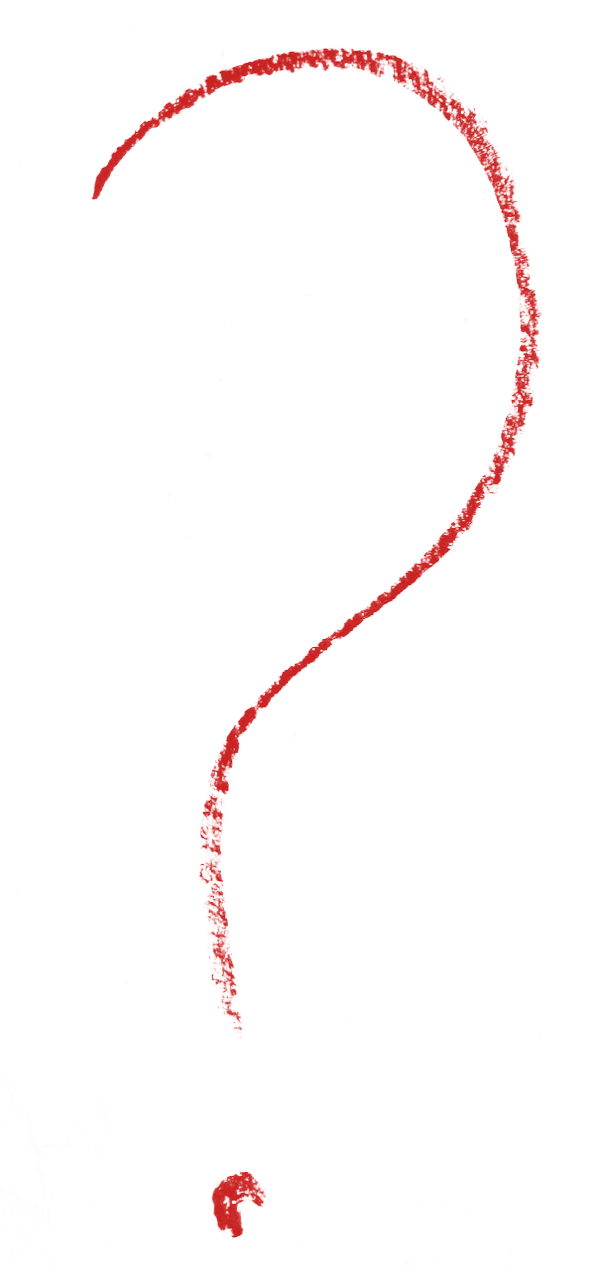
\includegraphics[height=0.6\textheight]{data/flickr/questionmark-alertred}
    \end{minipage}
    \hfill
    \begin{minipage}{0.56\textwidth}
        \centering
        \begin{block}{Construction}
            \begin{itemize}
                \item $f_k(x) \coloneqq\ $?
                \item Key schedule?
                \item $\mathcal{O}(n)$ rounds?
            \end{itemize}
        \end{block}
        \vspace{5pt}
        Theoretical vs.\ practical constructions
    \end{minipage}
    }
    \only<1->{\note{\begin{itemize}
        \item Sounds all very great.
        \item So from a practitioners point of view the natural next point is: lets implement it.
    \end{itemize}}}
    \only<2->{\note{\begin{itemize}
        \item But uggh\dots
        \item How does this Boolean function $f_k$ actually looks like?
        \item What about a key schedule? How do we derive the round keys?
        \item And how many are $\mathcal{O}(n)$ rounds?
    \end{itemize}
    \begin{itemize}
        \item So, from a theoretical point of view we have a nice construction.
        \item But from a practical point of view it is basically useless.
    \end{itemize}
    \begin{itemize}
        \item OK, let us fix this.
    \end{itemize}}
    }
\end{frame}

\section{Generic Analysis}
\begin{frame}{Generic Analysis}{On the number of rounds}
    \vspace{-20pt}
    \begin{minipage}[t][85pt][t]{0.47\textwidth}
        \begin{block}{Observation\vpPp}
            \begin{itemize}
                \item The ciphertext is the plaintext plus a subset of the round keys:
                    \begin{equation*}
                        y = x + \sum_{i=1}^{r} \lambda_i k_i
                    \end{equation*}
                \item For pairs $x_i, y_i$: $\Span \set{x_i + y_i} \subseteq \Span \set{k_j}$.
            \end{itemize}
            \vspace{2pt}
        \end{block}
    \end{minipage}
    \hfill
    \begin{minipage}[t][85pt][t]{0.47\textwidth}
        \visible<2->{%
        \begin{alertblock}{Distinguishing Attack for $r < n$ rounds\vpPp}
            \vspace{2pt}
            There is an $u \in \F_2^n \setminus \set{0}$, \st/ $\angles{u, x} = \angles{u, y}$ holds always:
            \begin{align*}
                        &\angles{u, y} = \angles{u, x + \sum \lambda_i k_i} \\
                        =\ &\angles{u, x} + \angles{u, \sum \lambda_i k_i} = \angles{u, x} + 0
                    \end{align*}
            for all $u \in \Span\set{k_1, \ldots, k_r}^\perp \neq \set{0}$
            \vspace{3pt}
        \end{alertblock}
        }
    \end{minipage}

    \vspace{50pt}

    \begin{minipage}{0.985\textwidth}
    \visible<3->{%
    \begin{exampleblock}{Rationale 1}
        Any instance must iterate at least n rounds; any set of n consecutive keys should be linearly indp.\vphantom{$\frac{1}{2}$}
    \end{exampleblock}
    }
    \end{minipage}
\end{frame}

\begin{frame}{Generic Analysis}{On the Boolean functions $f$}
    \centering

    A bit out of the blue sky, but:

    \begin{exampleblock}{Rationale 2}
        For any instance, $f_{k}$ has to depend on all bits, and for any $\delta \in \F_2^n:\ \Pr\bracket{f_k(x) = f_k(x + \delta)} \approx \frac{1}{2}$.
    \end{exampleblock}
\end{frame}

\begin{frame}{A genus of the WSN family: BISON}
    \centering
    \begin{exampleblock}{Rationale 1}
        Any instance must iterate at least n rounds; any set of n consecutive keys should be linearly indp.\vphantom{$\frac{1}{2}$}
    \end{exampleblock}
    \begin{exampleblock}{Rationale 2}
        For any instance, $f_{k}$ has to depend on all bits, and for any $\delta \in \F_2^n:\ \Pr\bracket{f_k(x) = f_k(x + \delta)} \approx \frac{1}{2}$.
    \end{exampleblock}
    \begin{block}{Generic properties of {\textbf{B}ent wh\textbf{I}tened \textbf{S}wap \textbf{O}r \textbf{N}ot}}
        \vspace{5pt}
        \begin{minipage}{0.51\textwidth}
        \begin{itemize}
            \item \only<1>{At least $n$ iterations of the round function}
                  \only<2>{\textcolor{alertred}{At least $n$ iterations of the round function}}
            \item Consecutive round keys linearly independent
        \end{itemize}
        \end{minipage}
        \begin{minipage}{0.44\textwidth}
        \begin{itemize}
            \item \only<1>{The round function depends on all bits}
                  \only<2>{\textcolor{alertred}{The round function depends on all bits}}
            \item $\forall \delta :\ \Pr\bracket{f_k(x) = f_k(x + \delta)} = \frac{1}{2}$ (\emph{bent})
        \end{itemize}
        \end{minipage}
        \vspace{5pt}
    \end{block}
    \visible<2->{%
        \vfill
        \begin{minipage}{0.47\textwidth}
            \centering
            \textcolor{alertred}{Rational 1 \& 2: WSN is \emph{slow} in practice!}
        \end{minipage}
        \hfill
        \begin{minipage}{0.47\textwidth}
            \centering
            But what about\\
            \Large
            Differential Cryptanalysis?
        \end{minipage}
        \vfill
    }
\end{frame}

\section{Differential Analysis}
\begin{frame}{Differential Cryptanalysis}{Primer}
    \centering
    \begin{tikzpicture}
    \tikzfading[name=fade out, inner color=transparent!0, outer color=transparent!100]
    \only<1>{%
        \node (f0) at ($0*(5cm,0)$) [minimum size=4cm, minimum height=5cm, rounded corners=1ex,fill=black!80!white,draw] {{\sc \textcolor{white}{Enc}}};
        \node (m0) [above=10pt of f0.north] {$p$};
        \node (k0) [left=10pt of f0.west] {$k$};
        \node (c0) [below=10pt of f0.south] {$c$\vphantom{$^\prime$}};
        \draw[-latex, thick] (m0) -- (f0);
        \draw[-latex, thick] (k0) -- (f0);
        \draw[-latex, thick] (f0) -- (c0);

        \node (f1) at ($1*(5cm,0)$) [minimum size=4cm, minimum height=5cm, rounded corners=1ex,fill=black!80!white,draw] {{\sc \textcolor{white}{Enc}}};
        \node (m1) [above=10pt of f1.north] {$p^\prime$};
        \node (k1) [right=10pt of f1.east] {$k$};
        \node (c1) [below=10pt of f1.south] {$c^\prime$};
        \draw[-latex, thick] (m1) -- (f1);
        \draw[-latex, thick] (k1) -- (f1);
        \draw[-latex, thick] (f1) -- (c1);

        \node (xor-in) [right=57.5pt of m0] {$\oplus$};
        \node (xor-out) [right=57.5pt of c0] {$\oplus$};
        \node (delta-in) [right=80pt of m1] {$= \textcolor{alertred}{\alpha}$};
        \node (delta-out) [right=80pt of c1] {$= \textcolor{alertred}{\beta}$};
        \draw[-latex, thick, dashed, color=alertred] (delta-in)+(4.5pt, -5pt) -- +(4.5pt, -172pt);
    }
    \only<2->{%
        \begin{scope}[opacity=0.2]
        \node (f0) at ($0*(5cm,0)$) [minimum size=4cm, minimum height=5cm, rounded corners=1ex,fill=white,draw] {{\sc Enc}};
        \node (m0) [above=10pt of f0.north] {$p$};
        \node (k0) [left=10pt of f0.west] {$k$};
        \node (c0) [below=10pt of f0.south] {$c$\vphantom{$^\prime$}};
        \draw[-latex, thick] (m0) -- (f0);
        \draw[-latex, thick] (k0) -- (f0);
        \draw[-latex, thick] (f0) -- (c0);

        \node (f1) at ($1*(5cm,0)$) [minimum size=4cm, minimum height=5cm, rounded corners=1ex,fill=white,draw] {{\sc Enc}};
        \node (m1) [above=10pt of f1.north] {$p^\prime$};
        \node (k1) [right=10pt of f1.east] {$k$};
        \node (c1) [below=10pt of f1.south] {$c^\prime$};
        \draw[-latex, thick] (m1) -- (f1);
        \draw[-latex, thick] (k1) -- (f1);
        \draw[-latex, thick] (f1) -- (c1);

        \node (xor-in) [right=57.5pt of m0] {$\oplus$};
        \node (xor-out) [right=57.5pt of c0] {$\oplus$};
        \node (delta-in) [right=80pt of m1] {$= \textcolor{alertred}{\alpha}$};
        \node (delta-out) [right=80pt of c1] {$= \textcolor{alertred}{\beta}$};
        \draw[-latex, thick, dashed, color=alertred] (delta-in)+(4.5pt, -5pt) -- +(4.5pt, -172pt);
        \end{scope}
    }

    \visible<2>{%
        \fill [fill=white, opacity=0.8, rounded corners=1ex] (0, 3.6) rectangle (4.5, -3.4);
        \node (diff-char) [below=-22pt of xor-in, xshift=-6pt] {\includegraphics[height=0.8\textheight]{data/differential-characteristic}};
    }
    \visible<3>{%
        \fill [fill=white, opacity=0.8, rounded corners=1ex] (0, 3.6) rectangle (4.5, -3.4);
        \node (diff) [below=-22pt of xor-in, xshift=-6pt] {\includegraphics[height=0.8\textheight]{data/differential}};
    }
    \end{tikzpicture}
\end{frame}

\begin{frame}{Differential Cryptanalysis}{One round}
    \vspace{-30pt}
    \begin{columns}
        \begin{column}{0.58\textwidth}
            \centering
            \vspace{30pt}
            \begin{block}{Proposition}
                %\centering
                For one round of \bison/
                the probabilities are:
                \begin{equation*}
                    \Prob\bracket{\alpha \to \beta} = \begin{cases*}
                        1           & if $\alpha = \beta = k$ or $\alpha = \beta = 0$\\
                        \frac{1}{2} & else if $\beta \in \set{\alpha, \alpha + k}$\\
                        0           & else
                    \end{cases*}
                \end{equation*}
            \end{block}
        \end{column}
        \begin{column}{0.40\textwidth}
            \vspace{40pt}
            \centering
            \vfill
            \visible<2->{%
                \begin{block}{Possible differences}
                    \vspace{-20pt}
                    \begin{alignat*}{5}
                                &x   &          &+ \hphantom{(} f_k(x)\ &                                \cdot &k \\
                        \oplus\ &x\  &+\ \alpha &                       &+\ f_k(x + \alpha) \hphantom{)} \cdot &k \\
                        =\      &    &\alpha\   &+ (f_k(x)\             &+\ f_k(x + \alpha))             \cdot &k
                    \end{alignat*}
                    \vspace{-17pt}
                \end{block}
            }
            \visible<3->{%
                \begin{block}{Remember}
                    \vspace{-10pt}
                    \begin{equation*}
                        \Pr\bracket{f_k(x) = f_k(x + \alpha)} = \frac{1}{2}
                    \end{equation*}
                    \vspace{-10pt}
                \end{block}
            }
            \vfill
        \end{column}
    \end{columns}
\end{frame}

\begin{frame}{Differential Cryptanalysis}{More rounds}
    Example differences over $r = 3$ rounds:\\[\baselineskip]

    \begin{center}
    \only<1>{%
    \begin{forest}
        [{$\alpha$}
            [{$\alpha$},
            edge label={node[midway,left,yshift=2mm,font=\scriptsize] {$\frac{1}{2}$}}
                [{$\alpha$}
                    [{$\alpha$}]
                    [{$\alpha + k_3$}]
                ]
                [{$\alpha + k_2$}
                    [{$\alpha + k_2$}]
                    [{$\alpha + k_2 + k_3$}]
                ]
            ]
            [{$\alpha + k_1$},
            edge label={node[midway,right,yshift=2mm,font=\scriptsize] {$\frac{1}{2}$}}
                [{$\alpha + k_1$},
                edge={thick},
                edge label={node[midway, left, yshift=2mm, font=\scriptsize] {$1$}}
                    [{$\alpha + k_1$}]
                    [{$\alpha + k_1 + k_3$}]
                ]
                [{$\alpha + k_1 + k_2$},
                edge={dotted, thick},
                edge label={node[midway, right, yshift=2mm, font=\scriptsize] {$0$}}
                    [{$\alpha + k_1 + k_2$}]
                    [{$\alpha + k_1 + k_2 + k_3$}]
                ]
            ]
        ]
    \end{forest}}\only<2>{%
    \begin{forest}
        [\textcolor{alertred}{$\alpha$}
            [\textcolor{alertred}{$\alpha$},
            edge={color=alertred, thick},
            edge label={node[midway,left,yshift=2mm,font=\scriptsize] {$\frac{1}{2}$}}
                [{$\alpha$}
                    [{$\alpha$}]
                    [{$\alpha + k_3$}]
                ]
                [\textcolor{alertred}{$\alpha + k_2$},
                edge={color=alertred, thick}
                    [\textcolor{alertred}{$\alpha + k_2$},
                    edge={color=alertred, thick}]
                    [{$\alpha + k_2 + k_3$}]
                ]
            ]
            [{$\alpha + k_1$},
            edge label={node[midway,right,yshift=2mm,font=\scriptsize] {$\frac{1}{2}$}}
                [{$\alpha + k_1$},
                edge={thick},
                edge label={node[midway, left, yshift=2mm, font=\scriptsize] {$1$}}
                    [{$\alpha + k_1$}]
                    [{$\alpha + k_1 + k_3$}]
                ]
                [{$\alpha + k_1 + k_2$},
                edge={dotted, thick},
                edge label={node[midway, right, yshift=2mm, font=\scriptsize] {$0$}}
                    [{$\alpha + k_1 + k_2$}]
                    [{$\alpha + k_1 + k_2 + k_3$}]
                ]
            ]
        ]
    \end{forest}}
    \vspace{20pt}

    \visible<2->{%
    For fixed \textcolor{alertred}{$\alpha$} and \textcolor{alertred}{$\beta$} there is only \emph{one} path!
    }
    \end{center}
\end{frame}

\section{The concrete Instance}
\begin{frame}{BISON}
    \centering
    \begin{minipage}{0.63\textwidth}
    \centering
    \begin{block}{A concrete species}
        \centering
        \vspace{2pt}
        
\includegraphics[height=0.7\textheight]{data/bison-logo}
    \end{block}
    \end{minipage}
\end{frame}

\begin{frame}{Addressing Rationale 1}{The Key Schedule}
    \vspace{-60pt}
    \begin{minipage}{0.985\textwidth}
    \begin{exampleblock}{Rationale 1}
        Any instance must iterate at least n rounds; any set of n consecutive keys should be linearly indp.\vphantom{$\frac{1}{2}$}
    \end{exampleblock}
    \end{minipage}

    \begin{minipage}[t][85pt][t]{0.47\textwidth}
        \begin{block}{Design Decisions}
            \begin{itemize}
                \item Choose number of rounds as $3 \cdot n$\\[5pt]
                \item Round keys derived from the state of LFSRs\\[5pt]
                \item Add round constants $c_i$ to $w_i$ round keys
            \end{itemize}
        \end{block}
    \end{minipage}
    \hfill
    \begin{minipage}[t][85pt][t]{0.47\textwidth}
        \begin{block}{Implications}
            \begin{itemize}
                \item Clocking an LFSR is cheap
                \item For an LFSR with irreducible feedback polynomial of degree $n$, every $n$ consecutive states are linearly independent
                \item Round constants avoid structural weaknesses
            \end{itemize}
        \end{block}
    \end{minipage}
\end{frame}

\begin{frame}{Addressing Rationale 2}{The Round Function}
    \vspace{-60pt}
    \begin{minipage}{0.985\textwidth}
    \begin{exampleblock}{Rationale 2}
        For any instance, the $f_{k}$ should depend on all bits, and for any $\delta \in \F_2^n:\ \Pr\bracket{f_k(x) = f_k(x + \delta)} \approx \frac{1}{2}$.
    \end{exampleblock}
    \end{minipage}

    \begin{minipage}[t][85pt][t]{0.47\textwidth}
        \begin{block}{Design Decisions}
            \begin{itemize}
                \item Choose $f_k : \F_2^n \to \F_2$ \st/
                      \begin{equation*}
                          \delta \in \F_2^n:\ \Pr\bracket{f_k(x) = f_k(x + \delta)} = \frac{1}{2},
                      \end{equation*}
                      that is, $f_k$ is a bent function.
                \item Choose the simplest bent function known:
                    \begin{equation*}
                        f_k(x, y) \coloneqq \angles{x, y}
                    \end{equation*}
            \end{itemize}
        \end{block}
    \end{minipage}
    \hfill
    \begin{minipage}[t][85pt][t]{0.47\textwidth}
        \begin{block}{Implications}
            \begin{itemize}
                \item Bent functions well studied\\[5pt]
                \item Bent functions only exists for even $n$\\[5pt]
                \item Instance not possible for every block length $n$
            \end{itemize}
        \end{block}
    \end{minipage}
\end{frame}

\section{Further Analysis}
\begin{frame}{Further Cryptanalysis}
    \begin{minipage}[t][70pt][t]{0.47\textwidth}
        \begin{block}{Linear Cryptanalysis\vpPp}
            For $r \geqslant n$ rounds, the correlation of any non-trivial linear trail for \bison/ is upper bounded by $2^{-\frac{n+1}{2}}$.
        \end{block}
    \end{minipage}
    \hfill
    \begin{minipage}[t][70pt][t]{0.47\textwidth}
        \begin{block}{Invariant Attacks\vpPp}
            For $r \geqslant n$ rounds, neither invariant subspaces nor nonlinear invariant attacks do exist for \bison/.
            \vspace{3pt}
        \end{block}
    \end{minipage}

    \begin{minipage}[t][70pt][t]{0.47\textwidth}
        \begin{block}{Zero Correlation\vpPp}
            For $r > 2n-2$ rounds, \bison/ does not exhibit any zero correlation linear hulls.
        \end{block}
    \end{minipage}
    \hfill
    \begin{minipage}[t][70pt][t]{0.47\textwidth}
        \begin{block}{Impossible Differentials\vpPp}
            For $r > n$ rounds, there are no impossible differentials for \bison/.
            \vspace{2pt}
        \end{block}
    \end{minipage}
\end{frame}

\begin{frame}{Implementation}{}
    TODO
\end{frame}

\begin{frame}{Conclusion/Questions}{Thank you for your attention!}
    \vspace{-80pt}
    \begin{minipage}[t][85pt][t]{0.47\textwidth}
        \begin{block}{\bison/\vpPp}
            \begin{itemize}
                \item A first instance of the WSN construction
                \item Good results for differential cryptanalysis
            \end{itemize}
        \end{block}
    \end{minipage}
    \hfill
    \begin{minipage}[t][85pt][t]{0.47\textwidth}
        \begin{block}{Open Problems}
            \begin{itemize}
                \item Construction for linear cryptanalysis
                \item Further analysis: division properties
            \end{itemize}
        \end{block}
    \end{minipage}

    \vspace{30pt}

    \begin{tikzpicture}[overlay]
        \node (thanks) at (2,0){};
        \draw[rotate=-7,line width=1.5pt,saphierblau,fill=gray!10]
             ($(thanks)-(1.5,.35)$) rectangle ($(thanks)+(1.5,.35)$)
             node[rotate=-7] at (thanks) {\textcolor{saphierblau}{\textbf{Thank you!}}};

        \node[right=100pt of thanks](questions){};
        \draw[rotate=3,line width=1.5pt,saphierblau,fill=gray!10]
             ($(questions)-(1.15,.35)$) rectangle ($(questions)+(1.15,.35)$)
             node[rotate=3] at (questions) {\textcolor{saphierblau}{\textbf{Questions?}}};

        \node[right=100pt of questions](eprint){};
        \draw[rotate=14,line width=1.5pt,saphierblau,fill=gray!10]
             ($(eprint)-(1.15,.35)$) rectangle ($(eprint)+(1.15,.35)$)
             node[rotate=14] at (eprint) {\textcolor{saphierblau}{\textcolor{gelbgruen}{\textbf{\href{https://ia.cr/2018/10111}{2018/1011}}}}};
    \end{tikzpicture}
\end{frame}

%\begin{frame}[allowframebreaks]{References}
%    %\begingroup
%    %    \scriptsize Title Image: \href{https://www.flickr.com/photos/bluetrailphoto/11095367173/in/photolist-hUsE72-7X4eFa-qd7u6B-eTa8pd-hiDwGF-cSTY2d-cSU6Ky-eSXJJt-cSTXLq-cSTUhq-arJDEr-cLkoTm-QWsSn3-6rEB3f-qAcyWm-r9yN4b-8Rh3wU-8msPC1-8VN8Qb-5Nyggn-bjUxdV-ent85f-DnwchP-cp6bmJ-wPFFSv-NhRU6s-cp69Kq-Nm4z1F-QnDuHm-HJcDrV-rEdDTc-MPZXa9-6bRMU6-KcegAy-aQCqMx-cp6d4L-X1c1Ym-aohLov-SSV7w-STFfT-atKAhj-qZXa1M-aecFP9-iRFVou-SSUb7-cp6dzu-cxr1qG-eJVbbv-oMb4qu-251se6T}{Blue Trail Photography: \enquote{Lords of the Plains (b\&w)}, \emph{flickr}}\\[1em]
%    %\endgroup
%    %\begingroup
%    %    \scriptsize Questionmark Image: \emph{flickr}\\[1em]
%    %\endgroup
%    \tiny
%    \printbibliography{}
%\end{frame}

\begin{frame}[plain]
    \centering
    \Huge
    \vspace{-1\baselineskip}
    Details
\end{frame}

\section{Specification}
\begin{frame}{\bison/}{Round Function}
    \vspace{-45pt}
    \begin{minipage}[t][150pt][t]{0.985\textwidth}
        \begin{block}{BISON's round function\vpPp}
            \centering
            \vspace{0.5\baselineskip}
            For round keys $k_i\in \F_2^n$ and $w_i\in \F_2^{n-1}$ the round function computes
            \begin{equation*}
                R_{k_i, w_i}(x) \coloneqq x + f_{b(i)} \parens{w_i + \Phi_{k_i}\parens{x}} \cdot k_i.
            \end{equation*}
            \flushleft
            where
            \begin{itemize}
                \item $\Phi_{k_i}$ and $f_{b(i)}$ are defined as
            \end{itemize}
            \vspace{-10pt}
            \begin{columns}
                \begin{column}{0.49\textwidth}
                    \begin{align*}
                        \Phi_k(x) : \F_2^n &\to \F_2^{n-1} \\
                        \Phi_k(x) &\coloneqq (x + x[i(k)] \cdot k)[j]_{\tower{1 \leqslant j \leqslant n}{j \neq i(k)}}
                    \end{align*}
                \end{column}
                \begin{column}{0.49\textwidth}
                    \begin{align*}
                        f_{b(i)} : \F_2^{\frac{n-1}{2}}\times \F_2^{\frac{n-1}{2}} &\to \F_2 \\
                        f_{b(i)}(x,y) &\coloneqq \angles{x,y} + b(i),
                    \end{align*}
                \end{column}
            \end{columns}
            \begin{itemize}
                \item and $b(i)$ is $0$ if $i \leqslant \frac{r}{2}$ and $1$ else.
            \end{itemize}
            \vspace{-0.25\baselineskip}
        \end{block}
    \end{minipage}
\end{frame}

\begin{frame}{\bison/}{Key Schedule\vpPp}
    \vspace{-45pt}
    \begin{minipage}[t][150pt][t]{0.985\textwidth}
        \begin{block}{BISON's key schedule}
            \vspace{0.5\baselineskip}
            Given
            \begin{itemize}
                \item primitive $p_k$, $p_w \in \F_2[x]$ with degrees $n$, $n-1$ and companion matrices $C_k$, $C_w$.
                \item master key $K = (k, w) \in \parens{\F_2^n \times \F_2^{n-1}} \setminus \set{0,0}$
            \end{itemize}
            The $i$th round keys are computed by
            \begin{align*}
                \ks_i : \F_2^n \times \F_2^{n-1} &\to \F_2^n \times \F_2^{n-1} \\
                \ks_i(k, w) &\coloneqq (k_i, c_i + w_i)
            \end{align*}
            where \begin{equation*}
                    k_i = \parens{C_k}^i k, \qquad
                    c_i = \parens{C_w}^{-i} e_1, \qquad
                    w_i = \parens{C_w}^i w.
                \end{equation*}
        \end{block}
    \end{minipage}
\end{frame}


\begin{frame}{Questions?}{Thank you for your attention!}
    \begin{columns}
        \begin{column}{0.58\textwidth}
            \begin{block}{Review}
                \begin{itemize}
                    \item Working as an engineer together with mathematicans can be fun\\
                        You can code, they\ldots{} can do math \Smiley{}
                    \item Even if you don't understand what you are implementing, you can get something working out of it
                    \item Eventually you'll understand the math \Ninja{}
                \end{itemize}
            \end{block}
        \end{column}
        \begin{column}{0.38\textwidth}
            \begin{figure}[!htb]
                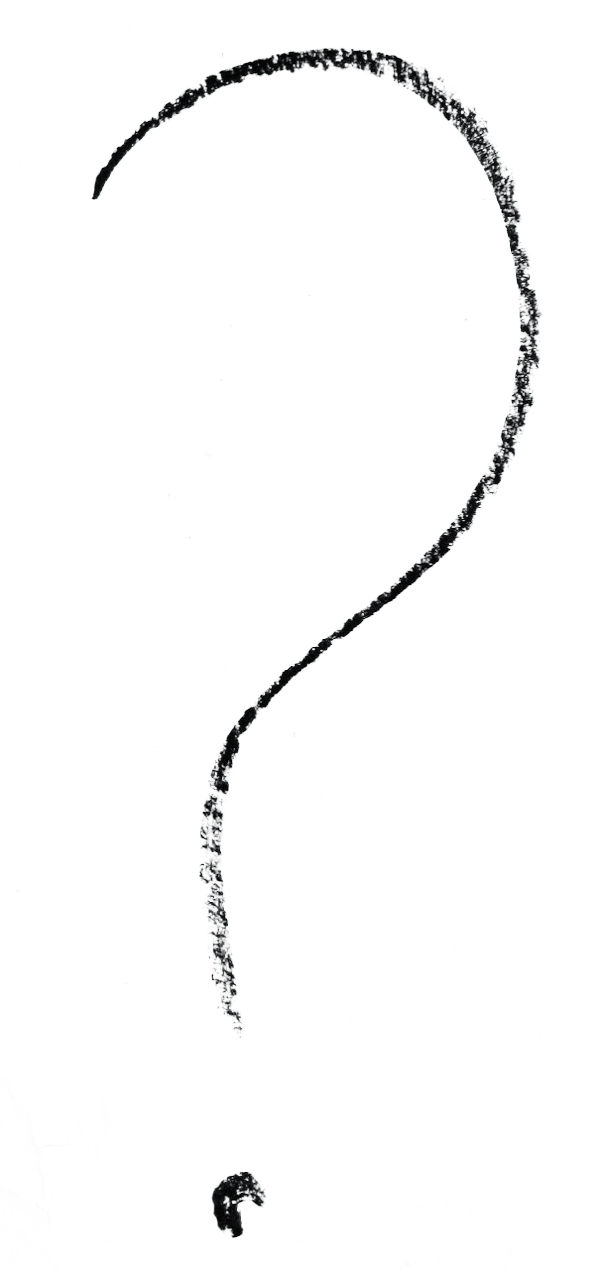
\includegraphics[height=50mm]{data/flickr/questionmark.png}
            \end{figure}
        \end{column}
    \end{columns}\blfootnote{\scriptsize Mainboard \& Questionmark Images: flickr}
\end{frame}

\begin{frame}[allowframebreaks]{References}
    \tiny
    \printbibliography{}
\end{frame}

\end{document}
